Jen has a jewelry box with $n$ rows and $m$ columns.
The rows are numbered from $1$ to $n$ from top to bottom, and the columns are numbered from $1$ to $m$ from left to right.
Each cell is identified by a pair $(x, y)$, which means it is located in the $x$-th row and the $y$-th column.

There are some jewels located in some cells of the box.
Each cell contains, at most, one jewel.
Surprisingly, no two jewels are located in adjacent cells.
In this problem, two cells are considered adjacent if they share an edge.

For some reason, Jen would like to form some pairs of jewels.
Each pair of jewels must be connected by a strand of rope, which may occupy some other cells of the jewelry box.
More formally, suppose a strand of rope connects jewels located at $(a_1,b_1)$ and $(a_k,b_k)$, and then the rope can be seen as a sequence of $k$ cells $(a_1,b_1),(a_2,b_2),\ldots,(a_k,b_k)$.
Each pair of consecutive cells must be adjacent, and all the $k$ cells should be distinct.
Due to aesthetics, no jewels should be attached to more than one rope, and no two ropes should occupy the same cell.

\newpage

\begin{figure}[h]
    \center
    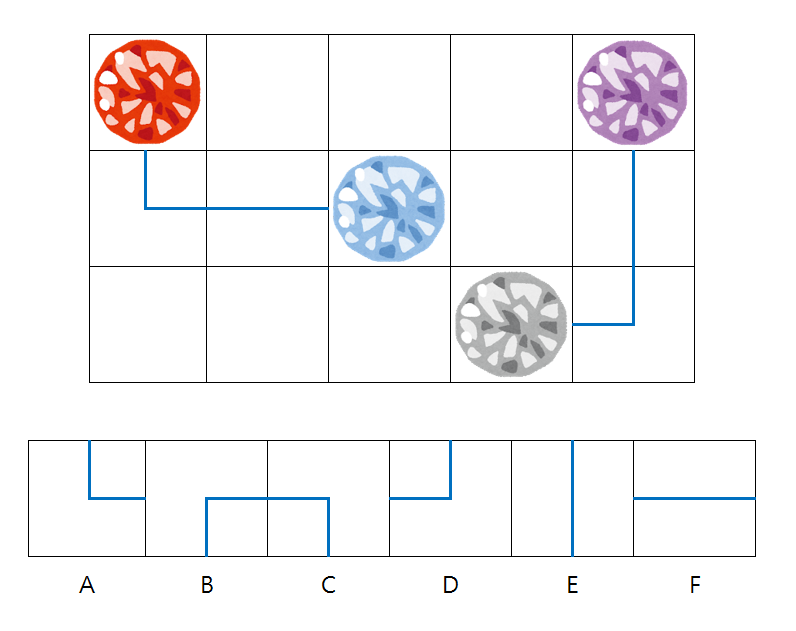
\includegraphics[width=0.5\textwidth]{image/jewel1.png}
    \caption{A valid configuration of jewels and ropes. There are $2$ pairs of jewels in the figure.}
    \end{figure}
    \begin{figure}[h]
    \center
    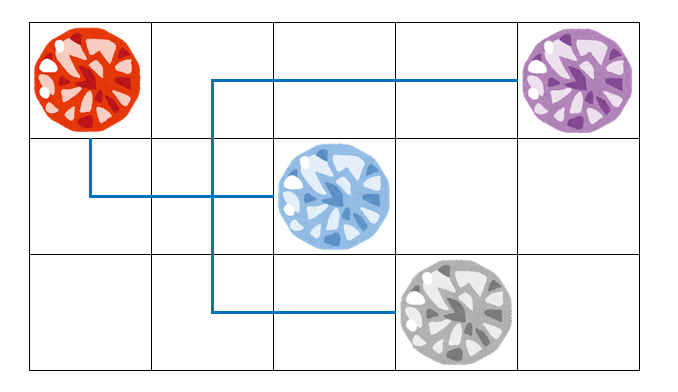
\includegraphics[width=0.5\textwidth]{image/jewel2.png}
    \caption{An invalid configuration of jewels and ropes because the two ropes share a common cell.}
    \end{figure}
Jen hopes to form as many pairs of jewels as possible. She also wonders about a way to place these strands of ropes. Can you help her out?